\documentclass[border=2pt]{standalone}
\usepackage{tikz}
\usetikzlibrary{arrows.meta,positioning,fit,calc}
\begin{document}
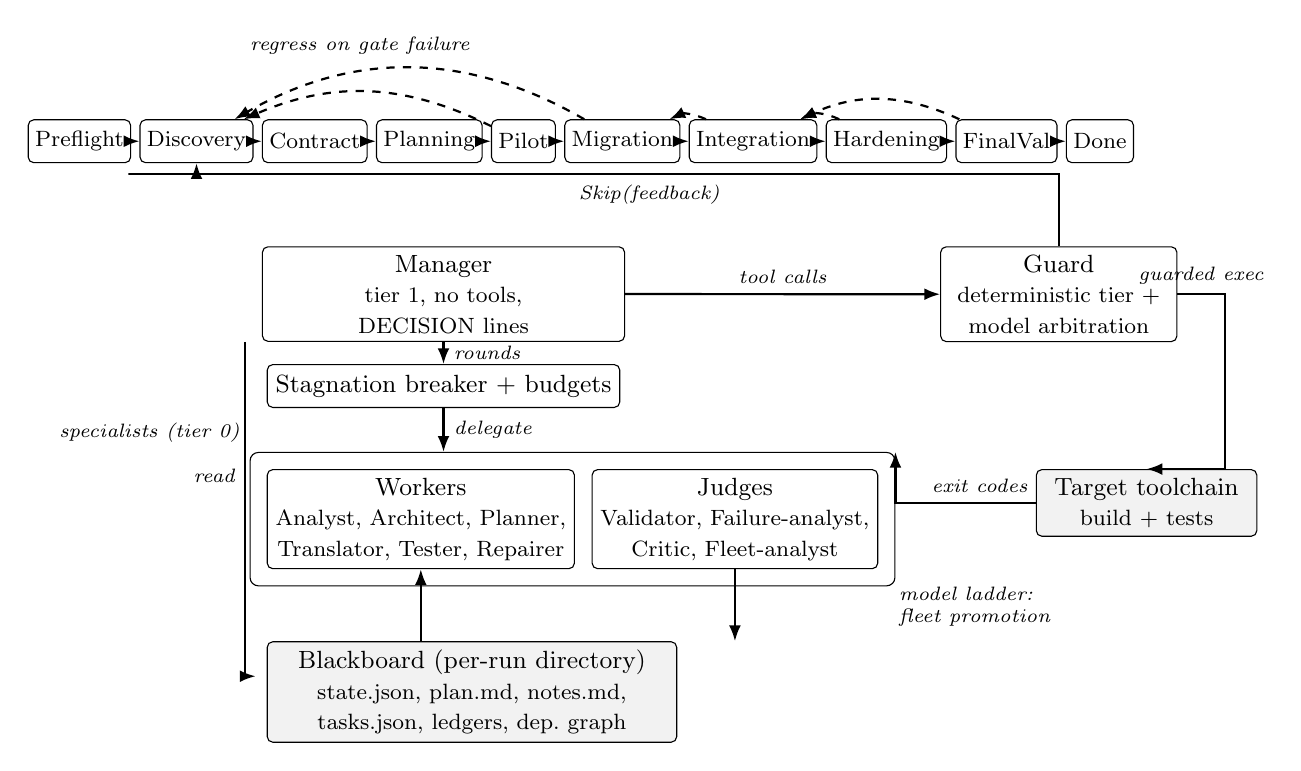
\begin{tikzpicture}[
  font=\small,
  role/.style={draw, rounded corners=2pt, align=center, inner sep=3pt, minimum height=1.55em},
  phase/.style={draw, rounded corners=2pt, align=center, inner sep=2.5pt, minimum height=1.55em, font=\footnotesize},
  cont/.style={draw, rounded corners=3pt, inner sep=6pt},
  arr/.style={-{Latex[length=2mm]}, thick},
  lab/.style={font=\scriptsize\itshape}
]

% Phase state machine (top strip)
\node[phase] (p0) {Preflight};
\node[phase, right=3pt of p0] (p1) {Discovery};
\node[phase, right=3pt of p1] (p2) {Contract};
\node[phase, right=3pt of p2] (p3) {Planning};
\node[phase, right=3pt of p3] (p4) {Pilot};
\node[phase, right=3pt of p4] (p5) {Migration};
\node[phase, right=3pt of p5] (p6) {Integration};
\node[phase, right=3pt of p6] (p7) {Hardening};
\node[phase, right=3pt of p7] (p8) {FinalVal};
\node[phase, right=3pt of p8] (p9) {Done};
\draw[arr] (p0) -- (p1);
\draw[arr] (p1) -- (p2);
\draw[arr] (p2) -- (p3);
\draw[arr] (p3) -- (p4);
\draw[arr] (p4) -- (p5);
\draw[arr] (p5) -- (p6);
\draw[arr] (p6) -- (p7);
\draw[arr] (p7) -- (p8);
\draw[arr] (p8) -- (p9);
% Legal regressions (curved, above)
\draw[arr, dashed] (p4) to[bend right=25] (p1);
\draw[arr, dashed] (p5) to[bend right=30] (p1);
\draw[arr, dashed] (p6) to[bend right=25] (p5);
\draw[arr, dashed] (p7) to[bend right=25] (p6);
\draw[arr, dashed] (p8) to[bend right=25] (p6);
\node[lab, anchor=south] at ($(p4.north)!0.5!(p1.north)+(0,20pt)$) {regress on gate failure};

% Manager loop (middle)
\node[role, below=30pt of p2.south west, anchor=north west, minimum width=46mm] (manager) {Manager\\ \footnotesize tier 1, no tools,\\ \footnotesize DECISION lines};
\node[role, below=8pt of manager] (breaker) {Stagnation breaker + budgets};
\draw[arr] (manager) -- node[lab, right]{rounds} (breaker);

% Guard
\node[role, right=40mm of manager.north east, anchor=north west, minimum width=30mm] (guard) {Guard\\ \footnotesize deterministic tier +\\ \footnotesize model arbitration};
\draw[arr] (manager.east) -- node[lab, above]{tool calls} (guard.west);
\draw[arr] (guard.north) |- node[lab, pos=0.72, below]{Skip(feedback)} ($(p1.south west)+(-4pt,-4pt)$) -| (p1.south);

% Specialists (two rows of roles)
\node[role, below=30pt of breaker.west, anchor=north west, minimum width=30mm] (workers) {Workers\\ \footnotesize Analyst, Architect, Planner,\\ \footnotesize Translator, Tester, Repairer};
\node[role, right=6pt of workers, minimum width=30mm] (judges) {Judges\\ \footnotesize Validator, Failure-analyst,\\ \footnotesize Critic, Fleet-analyst};

% Blackboard
\node[role, below=26pt of workers.south west, anchor=north west, minimum width=52mm, fill=gray!10] (blackboard) {Blackboard (per-run directory)\\ \footnotesize state.json, plan.md, notes.md,\\ \footnotesize tasks.json, ledgers, dep.\ graph};
\draw[arr] (blackboard.north -| workers.south) -- (workers.south);
\draw[arr] (judges.south) -- (blackboard.north -| judges.south);
\draw[arr] (manager.south west) +(-6pt,0) |- ($(blackboard.west)+(-4pt,2mm)$) node[lab, pos=0.2, left]{read};

% Container fits
\node[cont, fit=(workers)(judges), label={[lab]north west:specialists (tier 0)}] (specbox) {};

% Delegation arrow breaker -> specialists
\draw[arr] (breaker.south) -- node[lab, right]{delegate} (specbox.north -| breaker.south);

% Fleet ladder note (below judges, in free space)
\node[lab, align=left, anchor=north west] at ([xshift=4pt, yshift=-3pt]judges.south east) {model ladder:\\ fleet promotion};

% External toolchain
\node[role, right=20mm of judges.north east, anchor=north west, minimum width=28mm, fill=gray!10] (toolchain) {Target toolchain\\ \footnotesize build + tests};
\draw[arr] (guard.east) -- node[lab, above]{guarded exec} ($(guard.east)+(6mm,0)$) |- (toolchain.north);
\draw[arr] (toolchain.west) -| node[lab, pos=0.2, above]{exit codes} (specbox.north east);

\end{tikzpicture}
\end{document}
